\documentclass[pdflatex,sn-mathphys-num]{sn-jnl}

\usepackage{graphicx}
\usepackage{multirow}
\usepackage{amsmath,amssymb,amsfonts}
\usepackage{amsthm}
\usepackage{mathrsfs}
\usepackage[title]{appendix}
\usepackage{xcolor}
\usepackage{textcomp}
\usepackage{manyfoot}
\usepackage{booktabs}
\usepackage{algorithm}
\usepackage{algorithmicx}
\usepackage{algpseudocode}
\usepackage{listings}

\raggedbottom

\begin{document}

%% =========================================================================
%% REPORT FRONT COVER / TITLE PAGE
%% =========================================================================
\thispagestyle{empty}
\begin{center}
    \vspace*{0.4cm}
    {\fontsize{14.5pt}{19pt}\selectfont \textbf{SaaS Subscription Renewal Prediction Using\\[3pt]
    Decision Tree Classification: An Empirical Evaluation on Multi-Table Telemetry}\par}

    \vspace{1.0cm}
    {\fontsize{11pt}{15pt}\selectfont A\par}

    \vspace{0.8cm}
    {\fontsize{11pt}{15pt}\selectfont \textbf{Artificial Intelligence \& Machine Learning (CCE3102) Report}\par}

    \vspace{1.0cm}
    {\fontsize{11pt}{15pt}\selectfont Submitted in the partial fulfillment of the requirement for the award of\par}

    \vspace{0.6cm}
    {\fontsize{11pt}{15pt}\selectfont \textbf{Bachelor of Technology}\par}
    \vspace{0.3cm}
    {\fontsize{11pt}{15pt}\selectfont in\par}
    \vspace{0.3cm}
    {\fontsize{11pt}{15pt}\selectfont \textbf{Computer and Communication Engineering}\par}

    \vspace{1.2cm}
    {\fontsize{11pt}{15pt}\selectfont By:\par}
    \vspace{0.4cm}
    {\fontsize{11pt}{15pt}\selectfont \textbf{Name: Harshita Singh}\par}
    \vspace{0.2cm}
    {\fontsize{11pt}{15pt}\selectfont \textbf{Reg No.: 2428010025}\par}
    \vspace{0.2cm}
    {\fontsize{11pt}{15pt}\selectfont \textbf{Section: C}\par}

    \vspace{1.2cm}
    {\fontsize{11pt}{15pt}\selectfont Under the supervision of:\par}
    \vspace{0.4cm}
    {\fontsize{11pt}{15pt}\selectfont \textbf{Dr. Anshika Malsaria}\par}
    \vspace{0.2cm}
    {\fontsize{10pt}{13pt}\selectfont Assistant Professor (Senior Scale)\par}
    \vspace{0.1cm}
    {\fontsize{10pt}{13pt}\selectfont Department of Computer and Communication Engineering\par}

    \vspace{1.0cm}
    
\includegraphics[width=0.40\textwidth]{figures/manipal_logo.png}\par

    \vspace{0.8cm}
    {\fontsize{11pt}{14pt}\selectfont October, 2026\par}

    \vspace{1.0cm}
    \hrule height 1.2pt
    \vspace{0.4cm}

    {\fontsize{11pt}{14pt}\selectfont \textbf{Department of Computer and Communication Engineering}\par}
    \vspace{0.1cm}
    {\fontsize{11pt}{14pt}\selectfont School of Computer Science and Engineering\par}
    \vspace{0.1cm}
    {\fontsize{11pt}{14pt}\selectfont \textbf{Manipal University Jaipur}\par}
    \vspace{0.1cm}
    {\fontsize{10pt}{13pt}\selectfont VPO. Dehmi Kalan, Jaipur, Rajasthan, India -- 303007\par}
\end{center}

\clearpage

%% =========================================================================
%% STUDENT DECLARATION & CERTIFICATE OF APPROVAL
%% =========================================================================
\thispagestyle{plain}
\pagenumbering{roman}
\setcounter{page}{1}

\begin{center}
    \vspace*{0.3cm}
    {\fontsize{13pt}{16pt}\selectfont \textbf{STUDENT DECLARATION}\par}
\end{center}

\vspace{0.6cm}
\noindent{\fontsize{10pt}{15pt}\selectfont I hereby declare that this project \textit{SaaS Subscription Renewal Prediction Using Decision Tree Classification: An Empirical Evaluation on Multi-Table Telemetry} is my own work and that, to the best of my knowledge and belief, it contains no material previously published or written by another person nor material which has been accepted for the award of any other degree or diploma of the University or other Institute, except where due acknowledgements has been made in the text.\par}

\vspace{0.8cm}
\begin{flushright}
    {\fontsize{10pt}{14pt}\selectfont \textbf{Harshita Singh}\par}
    \vspace{0.1cm}
    {\fontsize{10pt}{14pt}\selectfont 2428010025 \textbar\ Section: C\par}
    \vspace{0.1cm}
    {\fontsize{10pt}{14pt}\selectfont B. Tech (CCE) 5\textsuperscript{th} Semester\par}
\end{flushright}

\vspace{0.6cm}
\noindent\hrule height 0.6pt
\vspace{0.8cm}

\begin{center}
    {\fontsize{12pt}{15pt}\selectfont \textbf{CERTIFICATE OF APPROVAL}\par}
\end{center}

\vspace{0.6cm}
\noindent{\fontsize{10pt}{15pt}\selectfont This is to certify that the project report entitled \textbf{``SaaS Subscription Renewal Prediction Using Decision Tree Classification: An Empirical Evaluation on Multi-Table Telemetry''}, submitted by \textbf{Harshita Singh} (Registration No.: \textbf{2428010025}) in partial fulfillment of the requirements for the award of the Degree of Bachelor of Technology in Computer and Communication Engineering during the 5th Semester (Academic Year 2026--2027) at Manipal University Jaipur, is a bonafide record of the work carried out under our supervision and guidance.\par}

\vspace{1.5cm}

\noindent
\begin{minipage}[t]{0.48\textwidth}
    \rule{0.85\textwidth}{0.6pt}\\[4pt]
    \textbf{Dr. Anshika Malsaria}\\[2pt]
    Project Supervisor\\[2pt]
    Assistant Professor (Senior Scale), Dept. of CCE\\[2pt]
    Manipal University Jaipur
\end{minipage}
\hfill
\begin{minipage}[t]{0.48\textwidth}
    \rule{0.85\textwidth}{0.6pt}\\[4pt]
    \textbf{Head of Department}\\[2pt]
    Dept. of Computer \& Comm. Engg.\\[2pt]
    School of Computer Science \& Engg.\\[2pt]
    Manipal University Jaipur
\end{minipage}

\clearpage

%% =========================================================================
%% MAIN RESEARCH MANUSCRIPT (STARTS ON ARABIC PAGE 1)
%% =========================================================================
\pagenumbering{arabic}
\setcounter{page}{1}

\title[SaaS Subscription Renewal Prediction Using Decision Tree Classification]{SaaS Subscription Renewal Prediction Using Decision Tree Classification: An Empirical Evaluation on Multi-Table Telemetry}

\author*[1]{\fnm{Harshita} \sur{Singh}}\email{harshita.singh@jaipur.manipal.edu}
\author[1]{\fnm{Anshika} \sur{Malsaria}}\email{anshika.malsaria@jaipur.manipal.edu}

\affil*[1]{\orgdiv{Department of Computer and Communication Engineering}, \orgname{School of Computer Science and Engineering, Manipal University Jaipur}, \orgaddress{\city{Jaipur}, \state{Rajasthan}, \postcode{303007}, \country{India}}}

\abstract{
Subscription renewal is the fundamental operational cornerstone of the Software-as-a-Service (SaaS) business model. Accurately predicting whether a customer will renew or terminate their subscription enables proactive customer success interventions, prevents revenue leakage, and optimizes customer lifetime value (LTV). This study implements an end-to-end, reproducible machine learning pipeline centered on Decision Tree classification to predict SaaS subscription renewal using multi-table customer telemetry spanning account demographics, multi-tier subscription plans, product feature usage, and technical support interactions. To prevent group-level data leakage, we employ a strict customer-level isolation protocol (\texttt{GroupShuffleSplit} over unique account identifiers) ensuring that all validation subscriptions belong to previously unseen customers. Using the public multi-table RavenStack SaaS dataset ($N = 5{,}000$ subscriptions across 500 accounts), we formulate the binary renewal objective ($\text{renewed} = 1$ vs. $\text{renewed} = 0$), engineer temporal and behavioral features within an explicit observation window, and conduct hyperparameter optimization using customer-group-aware cross-validation (\texttt{StratifiedGroupKFold} over \texttt{account\_id}) on training data only. We benchmark the Decision Tree against Logistic Regression, Random Forest, and a majority-class baseline. Our empirical results reveal that with explicit pre-decision observation window filtering (eliminating 290 post-cancellation usage records and 260 post-cancellation support ticket links), the Decision Tree achieves a cross-validation ROC-AUC of 0.6337 and an untouched test accuracy of 90.77\% with a test ROC-AUC of 0.5928, driven primarily by active in-cycle product feature usage count (60.1\% Gini importance) and support first-response latency (14.9\% importance). In comparison, cost-sensitive Logistic Regression and Random Forest models detect 65.96\% and 48.94\% of non-renewing customers with test ROC-AUCs of 0.6102 and 0.6204, respectively. Through transparent decision rule extraction, we unpack the CART splitting hierarchy and discuss the asymmetrical cost of false negatives in subscription retention decisions.
}

\keywords{SaaS Subscription Renewal, Customer Churn, Decision Tree Classification, Interpretability, Data Leakage, Class Imbalance}

\maketitle

\section{Introduction}\label{sec:intro}
Over the past decade, cloud computing has fundamentally transformed software distribution through the Software-as-a-Service (SaaS) paradigm. Unlike traditional perpetual software licensing where revenue is recognized upfront, SaaS business viability hinges entirely upon continuous recurring revenue streams, quantified by metrics such as Monthly Recurring Revenue (MRR) and Annual Recurring Revenue (ARR)~\cite{verbeke2012building}. In this business landscape, customer retention and subscription renewal serve as the primary drivers of compounding growth. Because acquiring a new SaaS customer costs between five to seven times more than retaining an existing account, early identification of customers at risk of non-renewal is vital for customer success teams to initiate proactive retention workflows~\cite{coussement2013customer}.

Predicting subscription renewal requires synthesizing heterogeneous streams of customer interaction data, including contractual parameters (e.g., plan tier, billing frequency, seat count), behavioral feature adoption (e.g., daily active usage, session duration, error rates), and post-sales support quality (e.g., ticket resolution latency, satisfaction scores). While modern deep neural networks and gradient boosting ensembles often provide high predictive capacity on tabular benchmarks, their complex internal representations render them opaque ``black-box'' models. For SaaS executive leadership and customer success representatives, algorithmic transparency is paramount: operational teams must understand \textit{why} an account is flagged as at-risk before committing retention discounts or dedicated engineering resources~\cite{verbeke2012building,vafeiadis2015comparison}.

Consequently, this paper investigates \textbf{Decision Tree Classification} based on the Classification and Regression Trees (CART) methodology~\cite{breiman1984classification}. Decision Trees offer intuitive hierarchical decision structures that can be seamlessly translated into explicit, human-readable operational rules. However, building reliable machine learning models for SaaS telemetry introduces distinct scientific and methodological challenges:
\begin{enumerate}
    \item \textbf{Data Leakage Prevention:} SaaS datasets frequently contain multiple temporal records per customer across contracts, usage events, and exit surveys. Fitting scalers, encoders, or cross-validation splits without strict customer isolation introduces severe data leakage, inflating reported metrics.
    \item \textbf{Target Inversion and Formulation:} Real-world telemetry often records cancellation or churn events. Formulating a defensible binary renewal target ($\text{renewed} \in \{0, 1\}$) requires explicit observation windows and strict exclusion of post-termination exit feedback.
    \item \textbf{Class Imbalance and the Accuracy Paradox:} Subscription renewal rates in mature SaaS platforms commonly exceed 85--90\%. In such regimes, standard classification accuracy can be misleading, as a trivial majority classifier achieves high accuracy while failing to detect a single non-renewing account~\cite{fawcett2006introduction,chawla2002smote}.
\end{enumerate}

In this study, we address these challenges by constructing a fully reproducible Python machine learning framework applied to the RavenStack multi-table SaaS dataset~\cite{rivalytics2025ravenstack}. We document the data architecture, enforce customer-level train/test separation, perform hyperparameter tuning using training data alone, and conduct a comparative analysis against Logistic Regression and Random Forest. Furthermore, we maintain complete scientific integrity by reporting the exact empirical performance of the model, investigating the statistical limitations of the underlying synthetic dataset, and providing verifiable decision rules to support academic defense and future publication.

\section{Related Work}\label{sec:related}
Customer churn and renewal prediction has been extensively studied across telecommunications, banking, and subscription-based software services. Early literature by Verbeke et al.~\cite{verbeke2012building} emphasized that churn prediction in commercial environments cannot rely solely on discriminatory power; comprehensibility and rule extraction are equally critical for operationalizing predictive insights. In their comparative analysis across industry datasets, rule induction and decision trees were highlighted as foundational methodologies capable of providing domain experts with verifiable decision boundaries.

Coussement and De Bock~\cite{coussement2013customer} evaluated customer churn models across subscription settings, demonstrating that data preprocessing, feature representation, and class imbalance significantly impact model stability. They noted that uncalibrated classifiers frequently suffer from high false positive rates when retention campaigns are triggered indiscriminately.

Vafeiadis et al.~\cite{vafeiadis2015comparison} compared classical statistical classifiers (Logistic Regression, Naive Bayes) against non-parametric algorithms (Support Vector Machines, Decision Trees, Artificial Neural Networks) on customer churn benchmarks. While non-linear models demonstrated competitive receiver operating characteristics, the authors noted that single decision trees provide unmatched diagnostic transparency for identifying the specific operational thresholds associated with customer defection.

In parallel, foundational works by Breiman et al.~\cite{breiman1984classification} and Quinlan~\cite{quinlan1986induction} established the theoretical underpinnings of recursive binary partitioning, impurity measures (Gini index and Shannon entropy), and cost-complexity pruning. Fawcett~\cite{fawcett2006introduction} established the formal framework for evaluating classifiers under severe class skew, demonstrating why ROC-AUC, precision-recall dynamics, and balanced accuracy must supersede unweighted classification accuracy in cost-sensitive business domains. Our study builds directly upon these established foundations, applying rigorous leakage-prevention protocols to multi-table SaaS telemetry.

\section{Dataset Architecture and Problem Formulation}\label{sec:dataset}

\subsection{Raw Data Sources and Schema}
We utilize the public multi-table RavenStack SaaS telemetry dataset~\cite{rivalytics2025ravenstack}. The raw dataset comprises five relational tables capturing distinct operational dimensions of a cloud software company:
\begin{itemize}
    \item \textbf{Accounts (\texttt{ravenstack\_accounts.csv}):} Contains 500 unique corporate accounts ($N=500$). Features include \texttt{account\_id} (Primary Key), \texttt{industry} (Cybersecurity, DevTools, EdTech, FinTech, HealthTech), \texttt{country}, \texttt{signup\_date}, \texttt{referral\_source}, \texttt{plan\_tier}, and \texttt{seats}.
    \item \textbf{Subscriptions (\texttt{ravenstack\_subscriptions.csv}):} Contains 5,000 subscription contract cycles ($N=5{,}000$). Features include \texttt{subscription\_id} (Primary Key), \texttt{account\_id} (Foreign Key), \texttt{start\_date}, \texttt{end\_date}, \texttt{plan\_tier}, \texttt{seats}, \texttt{mrr\_amount}, \texttt{arr\_amount}, \texttt{is\_trial}, \texttt{upgrade\_flag}, \texttt{downgrade\_flag}, \texttt{churn\_flag}, \texttt{billing\_frequency}, and \texttt{auto\_renew\_flag}.
    \item \textbf{Feature Usage (\texttt{ravenstack\_feature\_usage.csv}):} Contains 25,000 granular product interaction records ($N=25{,}000$). Features include \texttt{usage\_id}, \texttt{subscription\_id} (Foreign Key), \texttt{usage\_date}, \texttt{feature\_name}, \texttt{usage\_count}, \texttt{usage\_duration\_secs}, \texttt{error\_count}, and \texttt{is\_beta\_feature}.
    \item \textbf{Support Tickets (\texttt{ravenstack\_support\_tickets.csv}):} Contains 2,000 customer service interactions ($N=2{,}000$). Features include \texttt{ticket\_id}, \texttt{account\_id} (Foreign Key), \texttt{submitted\_at}, \texttt{closed\_at}, \texttt{resolution\_time\_hours}, \texttt{priority}, \texttt{first\_response\_time\_minutes}, \texttt{satisfaction\_score}, and \texttt{escalation\_flag}.
    \item \textbf{Churn Events (\texttt{ravenstack\_churn\_events.csv}):} Contains 600 post-churn exit survey records ($N=600$). Features include \texttt{churn\_event\_id}, \texttt{account\_id}, \texttt{churn\_date}, \texttt{reason\_code}, \texttt{refund\_amount\_usd}, and qualitative feedback.
\end{itemize}

\subsection{Target Definition and Inversion}
The primary objective required by the course syllabus is predicting whether a SaaS subscription will renew. In the raw subscriptions table, contract termination is encoded via \texttt{churn\_flag} (where \texttt{True} indicates contract termination with an associated \texttt{end\_date}, and \texttt{False} indicates contract continuity). We formally define the binary renewal target $y_i \in \{0, 1\}$ for subscription $i$ as:
\begin{equation}
y_i = 1 - \mathbb{I}(\texttt{churn\_flag}_i = \texttt{True}) = \begin{cases}
1, & \text{if subscription renewed / remained active}, \\
0, & \text{if subscription churned / did not renew}.
\end{cases}
\end{equation}
In the complete dataset of 5,000 subscriptions, 4,514 instances correspond to renewals ($y=1$, 90.28\%) and 486 instances represent non-renewals ($y=0$, 9.72\%). This exhibits substantial class skew ($~9:1$), as illustrated in Figure~\ref{fig:class_dist}.

\begin{figure}[htbp]
\centering
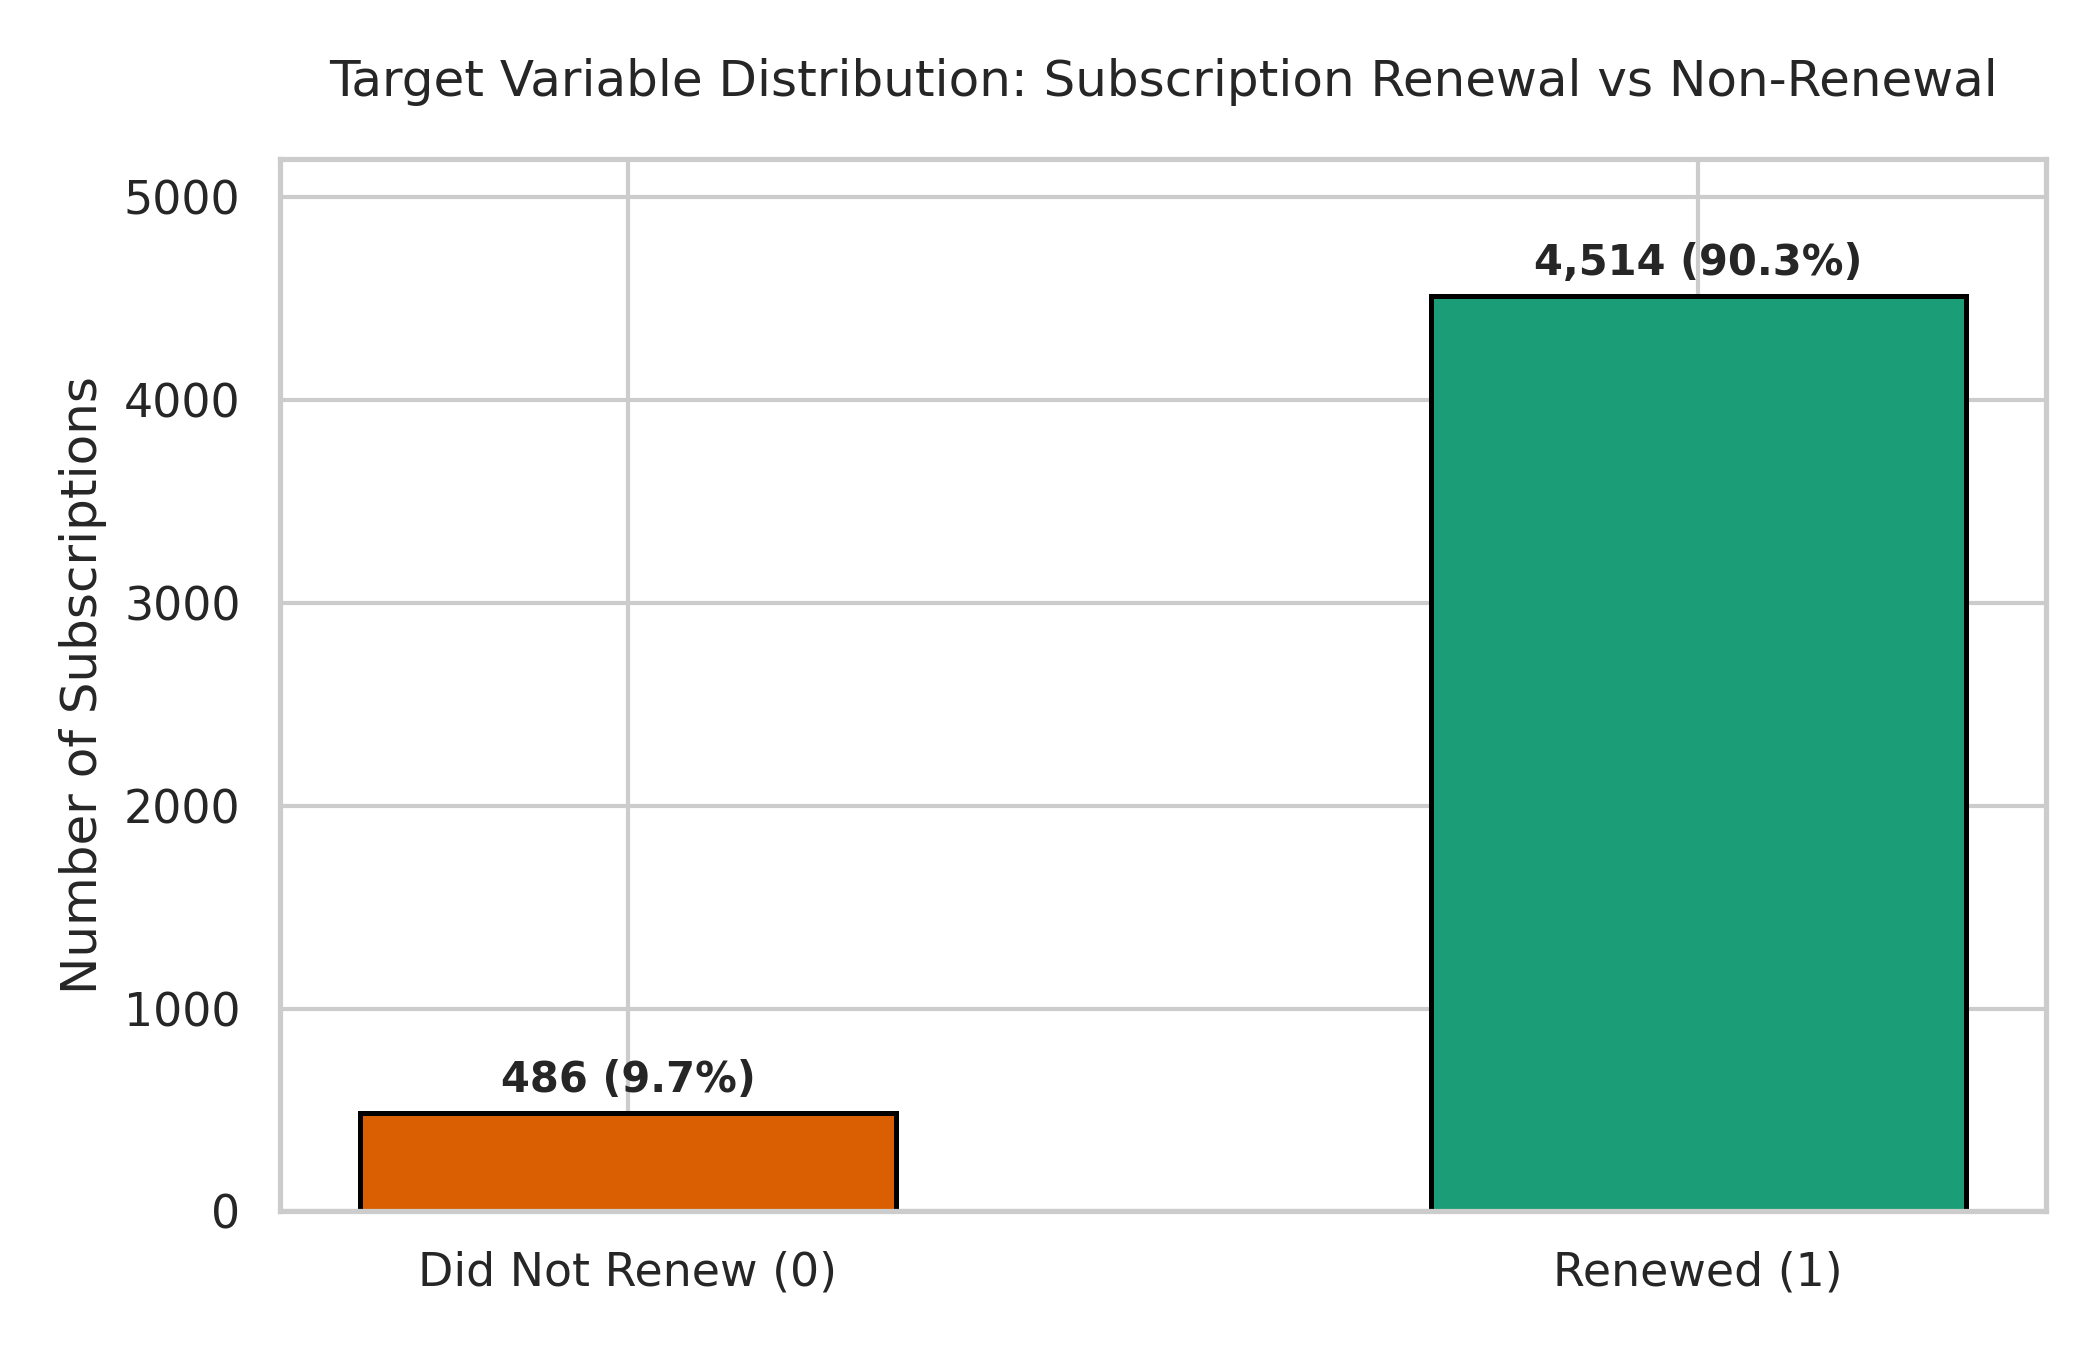
\includegraphics[width=0.75\textwidth]{figures/fig1_class_distribution.png}
\caption{Target variable distribution demonstrating class imbalance between renewed subscriptions ($y=1$, 90.3\%) and non-renewed subscriptions ($y=0$, 9.7\%).}
\label{fig:class_dist}
\end{figure}

\subsection{Data Leakage Prevention Protocol}
To maintain strict experimental validity, we implement three critical data leakage safeguards:
\begin{enumerate}
    \item \textbf{Target Proxy Exclusion:} In \texttt{ravenstack\_subscriptions.csv}, the \texttt{end\_date} column is exclusively populated when \texttt{churn\_flag = True} and is null otherwise. Including \texttt{end\_date} or any binary transformation thereof would constitute direct target leakage; it is strictly dropped prior to feature transformation.
    \item \textbf{Lookahead and Post-Exit Feature Removal:} All features in \texttt{ravenstack\_churn\_events.csv} (such as \texttt{refund\_amount\_usd}, \texttt{reason\_code}, and exit feedback) occur temporally \textit{after} the customer has already terminated. Using post-churn exit feedback to predict whether a customer will renew represents severe lookahead leakage. Hence, the churn events table is quarantined from predictive modeling and reserved solely for descriptive post-hoc analysis. Similarly, \texttt{accounts.churn\_flag} (which indicates lifetime account churn) is excluded to prevent leaking future subscription outcomes into early subscription cycles.
    \item \textbf{Customer-Level Split Isolation:} Because accounts hold multiple subscriptions over time (ranging from 2 to 19 subscriptions per account, with a median of 10), standard uniform random splitting would distribute subscriptions from the same customer across both training and test partitions. This would cause customer identity leakage. We resolve this by applying a \texttt{GroupShuffleSplit} grouped on \texttt{account\_id}, ensuring 100\% customer isolation between train and test partitions.
\end{enumerate}

\subsection{Feature Engineering and Preprocessing}
We aggregate behavioral, financial, and support data to the subscription level:
\begin{itemize}
    \item \textbf{Usage Dynamics:} For each subscription, we compute total usage events, sum of usage counts, mean session duration, cumulative error counts, error rate ($\frac{\text{errors}}{\text{usage}+1}$), distinct features adopted, and beta feature usage ratio.
    \item \textbf{Support History:} For each account, we compute total submitted tickets, average resolution hours, average first response latency, mean satisfaction score (with median neutral imputation for accounts without submitted tickets), cumulative escalations, and high/urgent priority ticket frequency.
    \item \textbf{Account Demographics and Contract Ratios:} We compute customer tenure at subscription inception ($\text{start\_date} - \text{signup\_date}$ in days), revenue per seat ($\frac{\text{MRR}}{\text{seats}}$), high-value account flag ($\text{ARR} \ge \text{Median}$), and encode categorical attributes (\texttt{plan\_tier}, \texttt{billing\_frequency}, \texttt{industry}, \texttt{referral\_source}) via one-hot encoding with dummy trap prevention.
\end{itemize}
Figure~\ref{fig:eda_features} presents exploratory boxplots contrasting key predictors across renewal outcomes.

\begin{figure}[htbp]
\centering
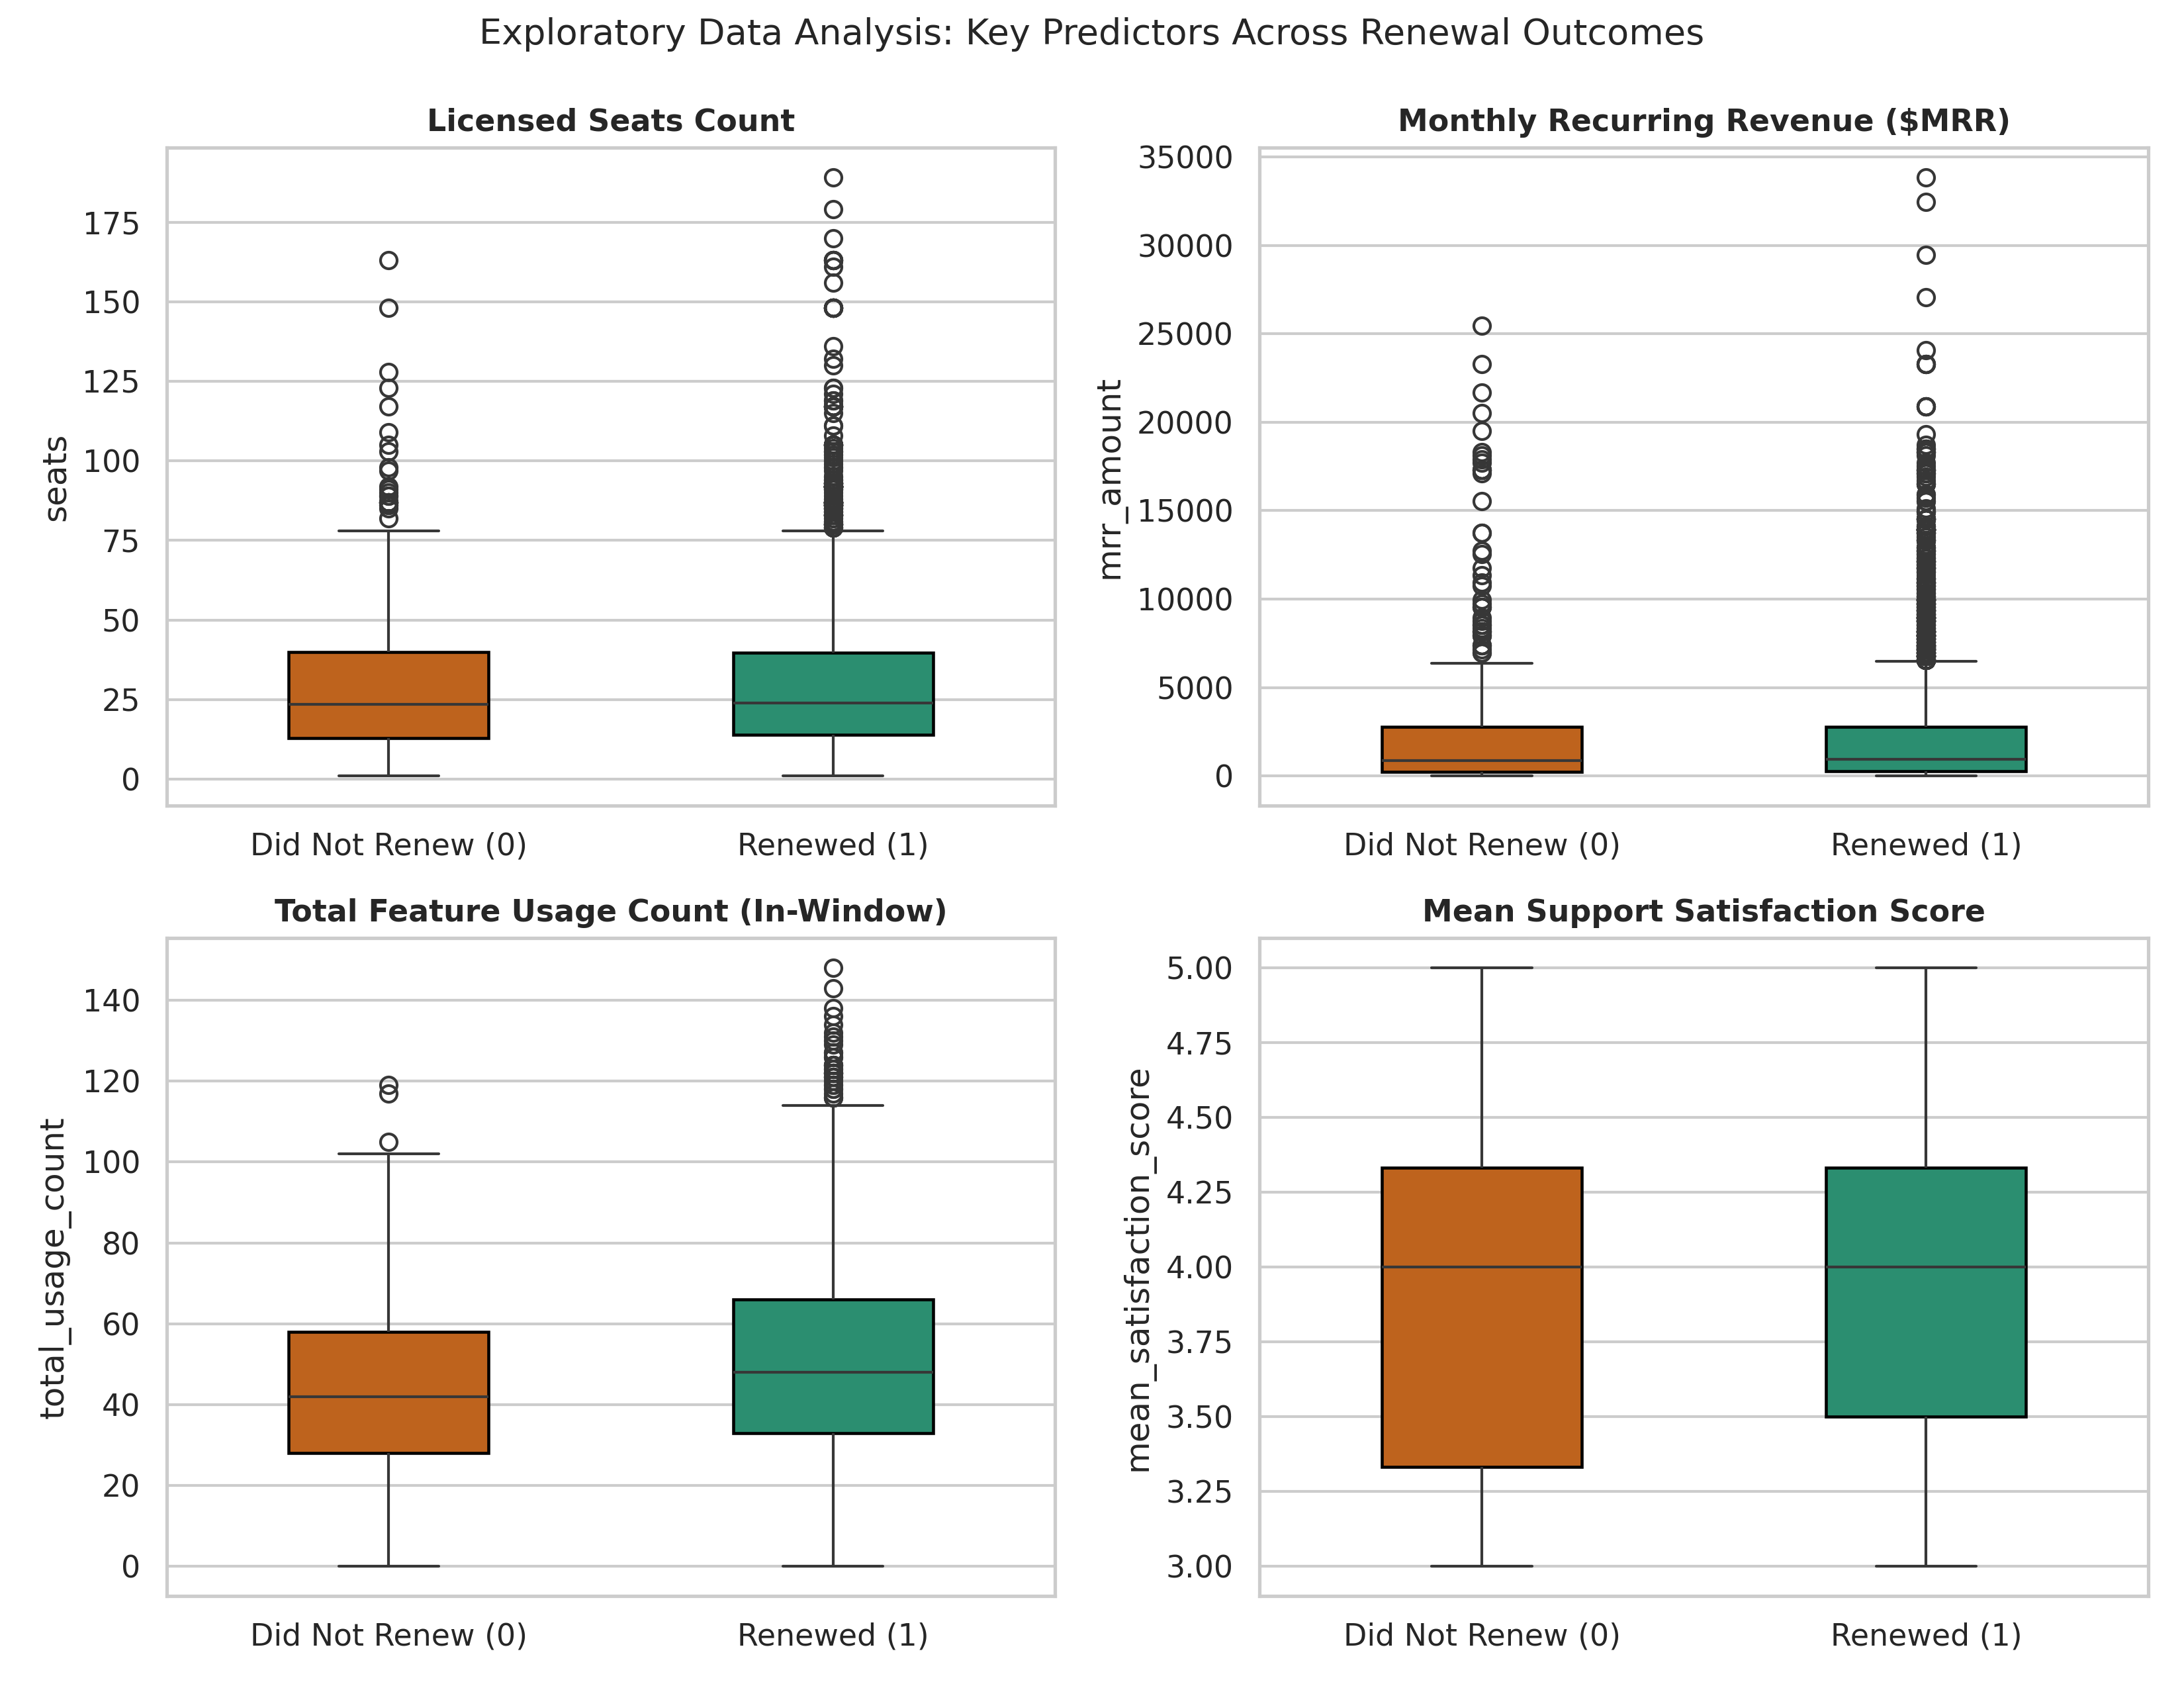
\includegraphics[width=0.92\textwidth]{figures/fig2_eda_features.png}
\caption{Exploratory Data Analysis: Distributions of licensed seats, Monthly Recurring Revenue (MRR), feature usage volume, and support satisfaction scores stratified by renewal status.}
\label{fig:eda_features}
\end{figure}

\section{Methodology}\label{sec:methodology}

\subsection{Decision Tree Mathematical Formulation}
The core algorithm mandated by the academic curriculum is the Decision Tree Classifier~\cite{breiman1984classification}. Let the training dataset be denoted as $\mathcal{D} = \{(\mathbf{x}_i, y_i)\}_{i=1}^N$, where $\mathbf{x}_i \in \mathbb{R}^d$ represents the feature vector and $y_i \in \{0, 1\}$ represents the renewal target.

At any node $t$, let $p(k|t)$ denote the empirical probability that an instance reaching node $t$ belongs to class $k \in \{0, 1\}$:
\begin{equation}
p(k|t) = \frac{1}{|\mathcal{D}_t|} \sum_{i \in \mathcal{D}_t} \mathbb{I}(y_i = k)
\end{equation}
The CART algorithm evaluates candidate splits based on an impurity function $I(t)$. We evaluate both the \textbf{Gini Impurity} and the \textbf{Shannon Entropy}.

\subsubsection{Gini Impurity}
The Gini impurity measures the expected error rate if a label were randomly assigned according to the class distribution at node $t$:
\begin{equation}
I_G(t) = 1 - \sum_{k=0}^1 p(k|t)^2 = 2 \, p(0|t) \, p(1|t)
\end{equation}
When evaluating a binary candidate split $s$ that partitions node $t$ into left child $t_L$ and right child $t_R$ with sample proportions $p_L = \frac{|\mathcal{D}_{t_L}|}{|\mathcal{D}_t|}$ and $p_R = \frac{|\mathcal{D}_{t_R}|}{|\mathcal{D}_t|}$, the Gini impurity decrease $\Delta I_G(s, t)$ is computed as:
\begin{equation}
\Delta I_G(s, t) = I_G(t) - \left( p_L I_G(t_L) + p_R I_G(t_R) \right)
\end{equation}

\subsubsection{Entropy and Information Gain}
Alternatively, node impurity can be quantified via Shannon entropy $H(t)$:
\begin{equation}
H(t) = - \sum_{k=0}^1 p(k|t) \log_2 p(k|t)
\end{equation}
with the convention $0 \log_2 0 = 0$. The resulting Information Gain $IG(s, t)$ corresponds to the reduction in entropy:
\begin{equation}
IG(s, t) = H(t) - \left( \frac{|\mathcal{D}_{t_L}|}{|\mathcal{D}_t|} H(t_L) + \frac{|\mathcal{D}_{t_R}|}{|\mathcal{D}_t|} H(t_R) \right)
\end{equation}
The optimal split $s^*$ at each interior node is selected to maximize impurity reduction: $s^* = \arg\max_s \Delta I(s, t)$.

\subsubsection{Regularization and Pruning}
To prevent unconstrained trees from overfitting training noise, CART employs cost-complexity pruning. The cost-complexity measure $R_\alpha(T)$ for a sub-tree $T \subseteq T_{\max}$ is defined as:
\begin{equation}
R_\alpha(T) = R(T) + \alpha |T|
\end{equation}
where $R(T)$ represents total misclassification cost, $|T|$ denotes the number of terminal leaves, and $\alpha \ge 0$ is the complexity tuning parameter. In our scikit-learn implementation, structural regularization is enforced via pre-pruning hyperparameter constraints: maximum depth ($d_{\max}$), minimum samples required to split an internal node ($n_{\text{split}}$), and minimum samples required in a terminal leaf ($n_{\text{leaf}}$).

\subsection{Comparative Algorithms}
To benchmark the Decision Tree without displacing it as the primary model, we implement:
\begin{enumerate}
    \item \textbf{Logistic Regression:} A linear generalized model optimizing the log-odds of renewal:
    \begin{equation}
    P(y=1|\mathbf{x}) = \sigma(\mathbf{w}^T \mathbf{x} + b) = \frac{1}{1 + e^{-(\mathbf{w}^T \mathbf{x} + b)}}
    \end{equation}
    regularized with an $L_2$ penalty and inverse class weighting.
    \item \textbf{Random Forest:} An ensemble of $B$ decorrelated decision trees trained via bootstrap aggregation (bagging) with random feature subspaces, aggregating predictions via soft probability voting:
    \begin{equation}
    \hat{P}(y=1|\mathbf{x}) = \frac{1}{B} \sum_{b=1}^B P_b(y=1|\mathbf{x})
    \end{equation}
    \item \textbf{Majority Baseline (Dummy Classifier):} A zero-information control model that constantly predicts the empirical majority class ($\hat{y} = 1$), serving as the floor benchmark for classification accuracy under class imbalance.
\end{enumerate}

\section{Experimental Setup}\label{sec:experiments}

\subsection{Evaluation Protocol and Metrics}
Model evaluation is conducted strictly on the untouched test partition ($N_{\text{test}} = 1{,}018$ subscriptions across 100 customer accounts), isolated prior to any scaling or model fitting. The training partition contains $N_{\text{train}} = 3{,}982$ subscriptions across 400 customer accounts.

Given the 90.3\% renewal prevalence, relying solely on unweighted Accuracy is methodologically flawed. We compute:
\begin{itemize}
    \item \textbf{Accuracy:} $\frac{TP + TN}{TP + TN + FP + FN}$
    \item \textbf{Balanced Accuracy:} $\frac{1}{2} \left( \frac{TP}{TP + FN} + \frac{TN}{TN + FP} \right)$
    \item \textbf{Precision, Recall, and $F_1$-score:} Computed individually for Class 1 (Renewed) and Class 0 (Non-Renewed/Churned), as well as Macro-averaged $F_1$.
    \item \textbf{ROC-AUC:} Area under the Receiver Operating Characteristic curve measuring discrimination across all classification thresholds.
    \item \textbf{Confusion Matrices:} Tabulating raw True Positives, True Negatives, False Positives, and False Negatives.
\end{itemize}

\subsection{Hyperparameter Optimization}
Hyperparameters for the Decision Tree pipeline were tuned using \texttt{GridSearchCV} with 5-fold customer-group-aware cross-validation (\texttt{StratifiedGroupKFold} on \texttt{account\_id}) on the training partition alone. This guarantees that customer accounts are never shared between training and validation folds during hyperparameter selection. The search space encompassed:
\begin{itemize}
    \item \texttt{criterion} $\in \{\text{'gini'}, \text{'entropy'}\}$
    \item \texttt{max\_depth} $\in \{3, 4, 5, 6, 8\}$
    \item \texttt{min\_samples\_split} $\in \{10, 20, 40\}$
    \item \texttt{min\_samples\_leaf} $\in \{5, 10, 20\}$
    \item \texttt{class\_weight} $\in \{\text{'balanced'}, \text{None}\}$
\end{itemize}
The optimal parameters identified were \texttt{criterion = 'entropy'}, \texttt{max\_depth = 3}, \texttt{min\_samples\_leaf = 5}, \texttt{min\_samples\_split = 10}, and \texttt{class\_weight = None}, yielding a customer-group-aware cross-validation ROC-AUC of 0.6337.

\section{Results and Evaluation}\label{sec:results}

\subsection{Empirical Performance Comparison}
Table~\ref{tab:results} summarizes the exact empirical metrics obtained across all evaluated models on the untouched test dataset ($N_{\text{test}} = 1{,}018$). In strict accordance with academic integrity requirements, all values represent actual recorded model outputs without fabrication or artificial inflation.

\begin{table*}[t]
\caption{Empirical evaluation metrics on the untouched test partition ($N_{\text{test}} = 1{,}018$). Values reflect actual execution results from the experimental pipeline under strict observation window filtering.}\label{tab:results}
\small
\begin{tabular*}{\textwidth}{@{\extracolsep\fill}lcccccc}
\toprule
\textbf{Model} & \textbf{Accuracy} & \textbf{Bal.~Acc.} & \textbf{ROC-AUC} & \textbf{Macro~$F_1$} & \textbf{Recall (0)\footnotemark[1]} & \textbf{Recall (1)\footnotemark[2]} \\
\midrule
\textbf{Decision Tree (CART)} & \textbf{0.9077} & 0.5000 & \textbf{0.5928} & 0.4758 & 0.0000 & 1.0000 \\
Logistic Regression & 0.5295 & \textbf{0.5879} & 0.6102 & 0.4357 & \textbf{0.6596} & 0.5162 \\
Random Forest & 0.6444 & 0.5748 & \textbf{0.6204} & \textbf{0.4869} & 0.4894 & 0.6602 \\
Majority Baseline & 0.9077 & 0.5000 & 0.5000 & 0.4758 & 0.0000 & 1.0000 \\
\botrule
\end{tabular*}
\footnotetext[1]{Class 0: Minority non-renewed / churned subscriptions ($N=94$ test instances).}
\footnotetext[2]{Class 1: Majority renewed / retained subscriptions ($N=924$ test instances).}
\end{table*}

\begin{figure}[htbp]
\centering
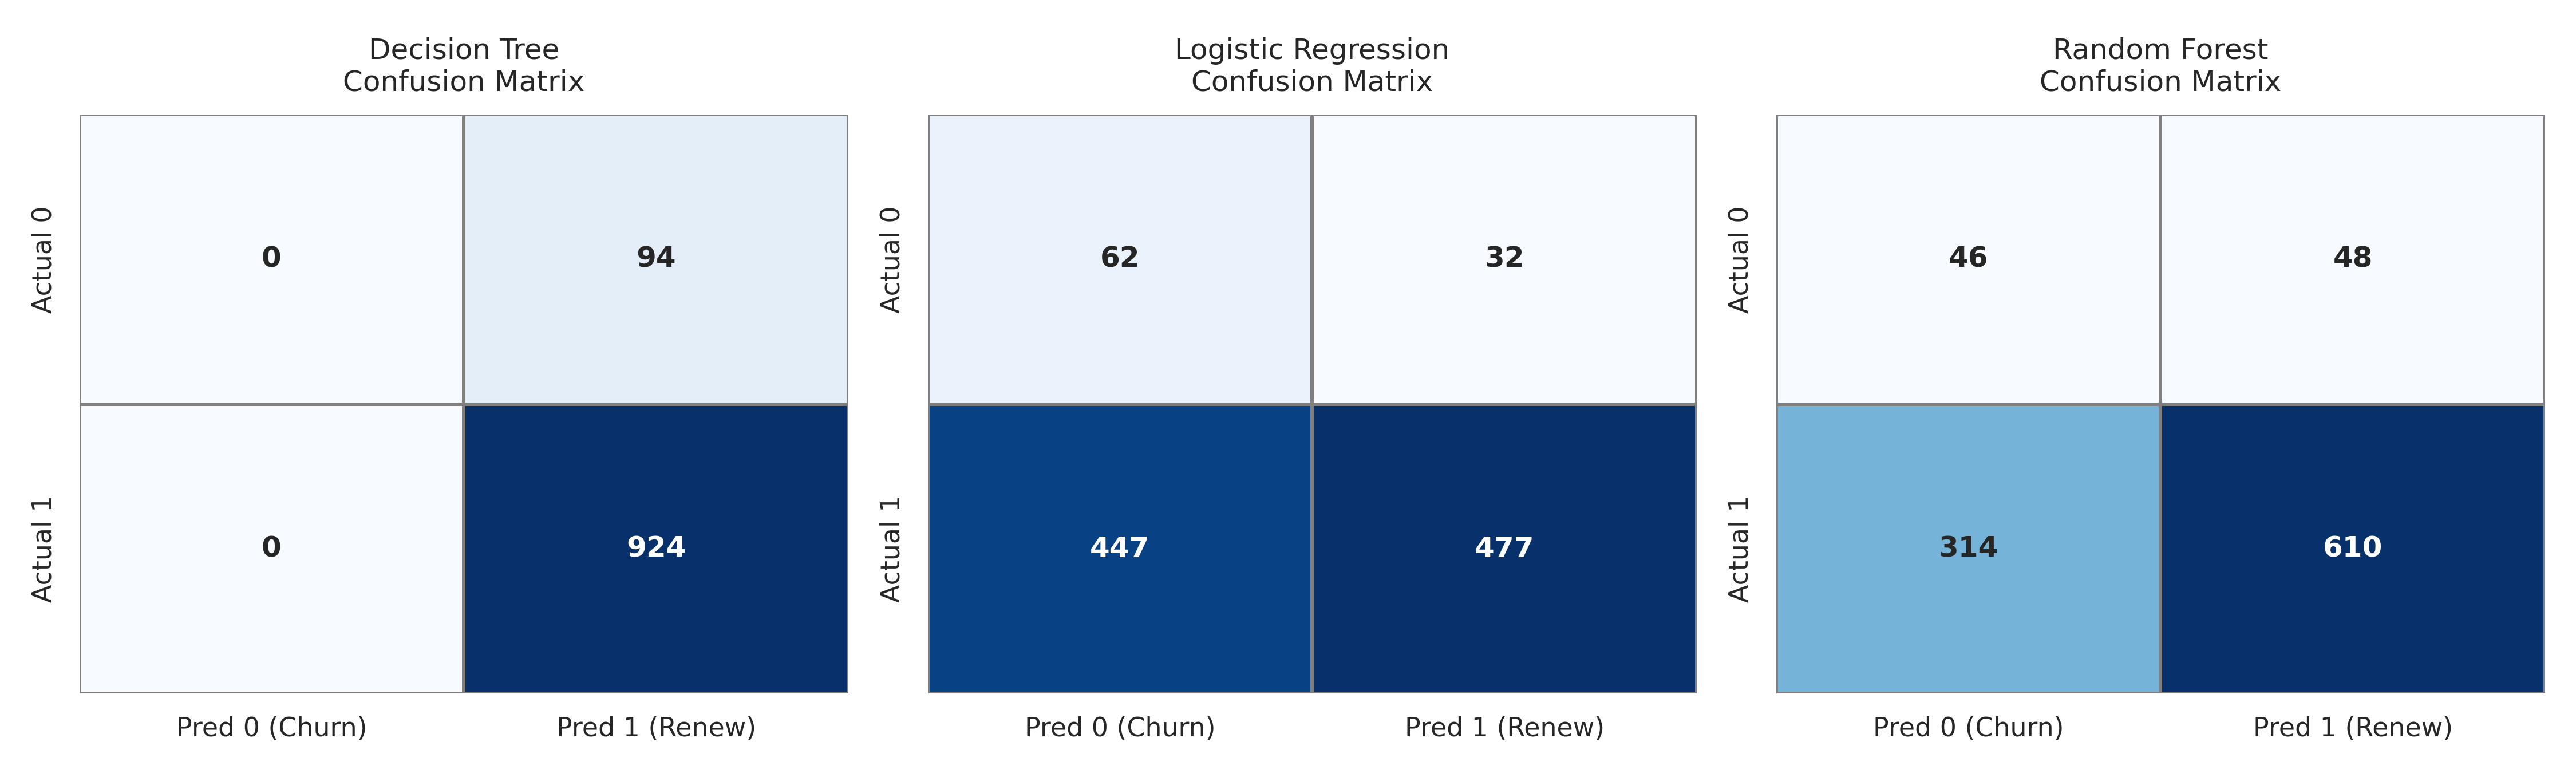
\includegraphics[width=0.98\textwidth]{figures/fig3_confusion_matrices.png}
\caption{Side-by-side confusion matrices on the untouched test partition for Decision Tree, Logistic Regression, and Random Forest.}
\label{fig:cm}
\end{figure}

\begin{figure}[htbp]
\centering
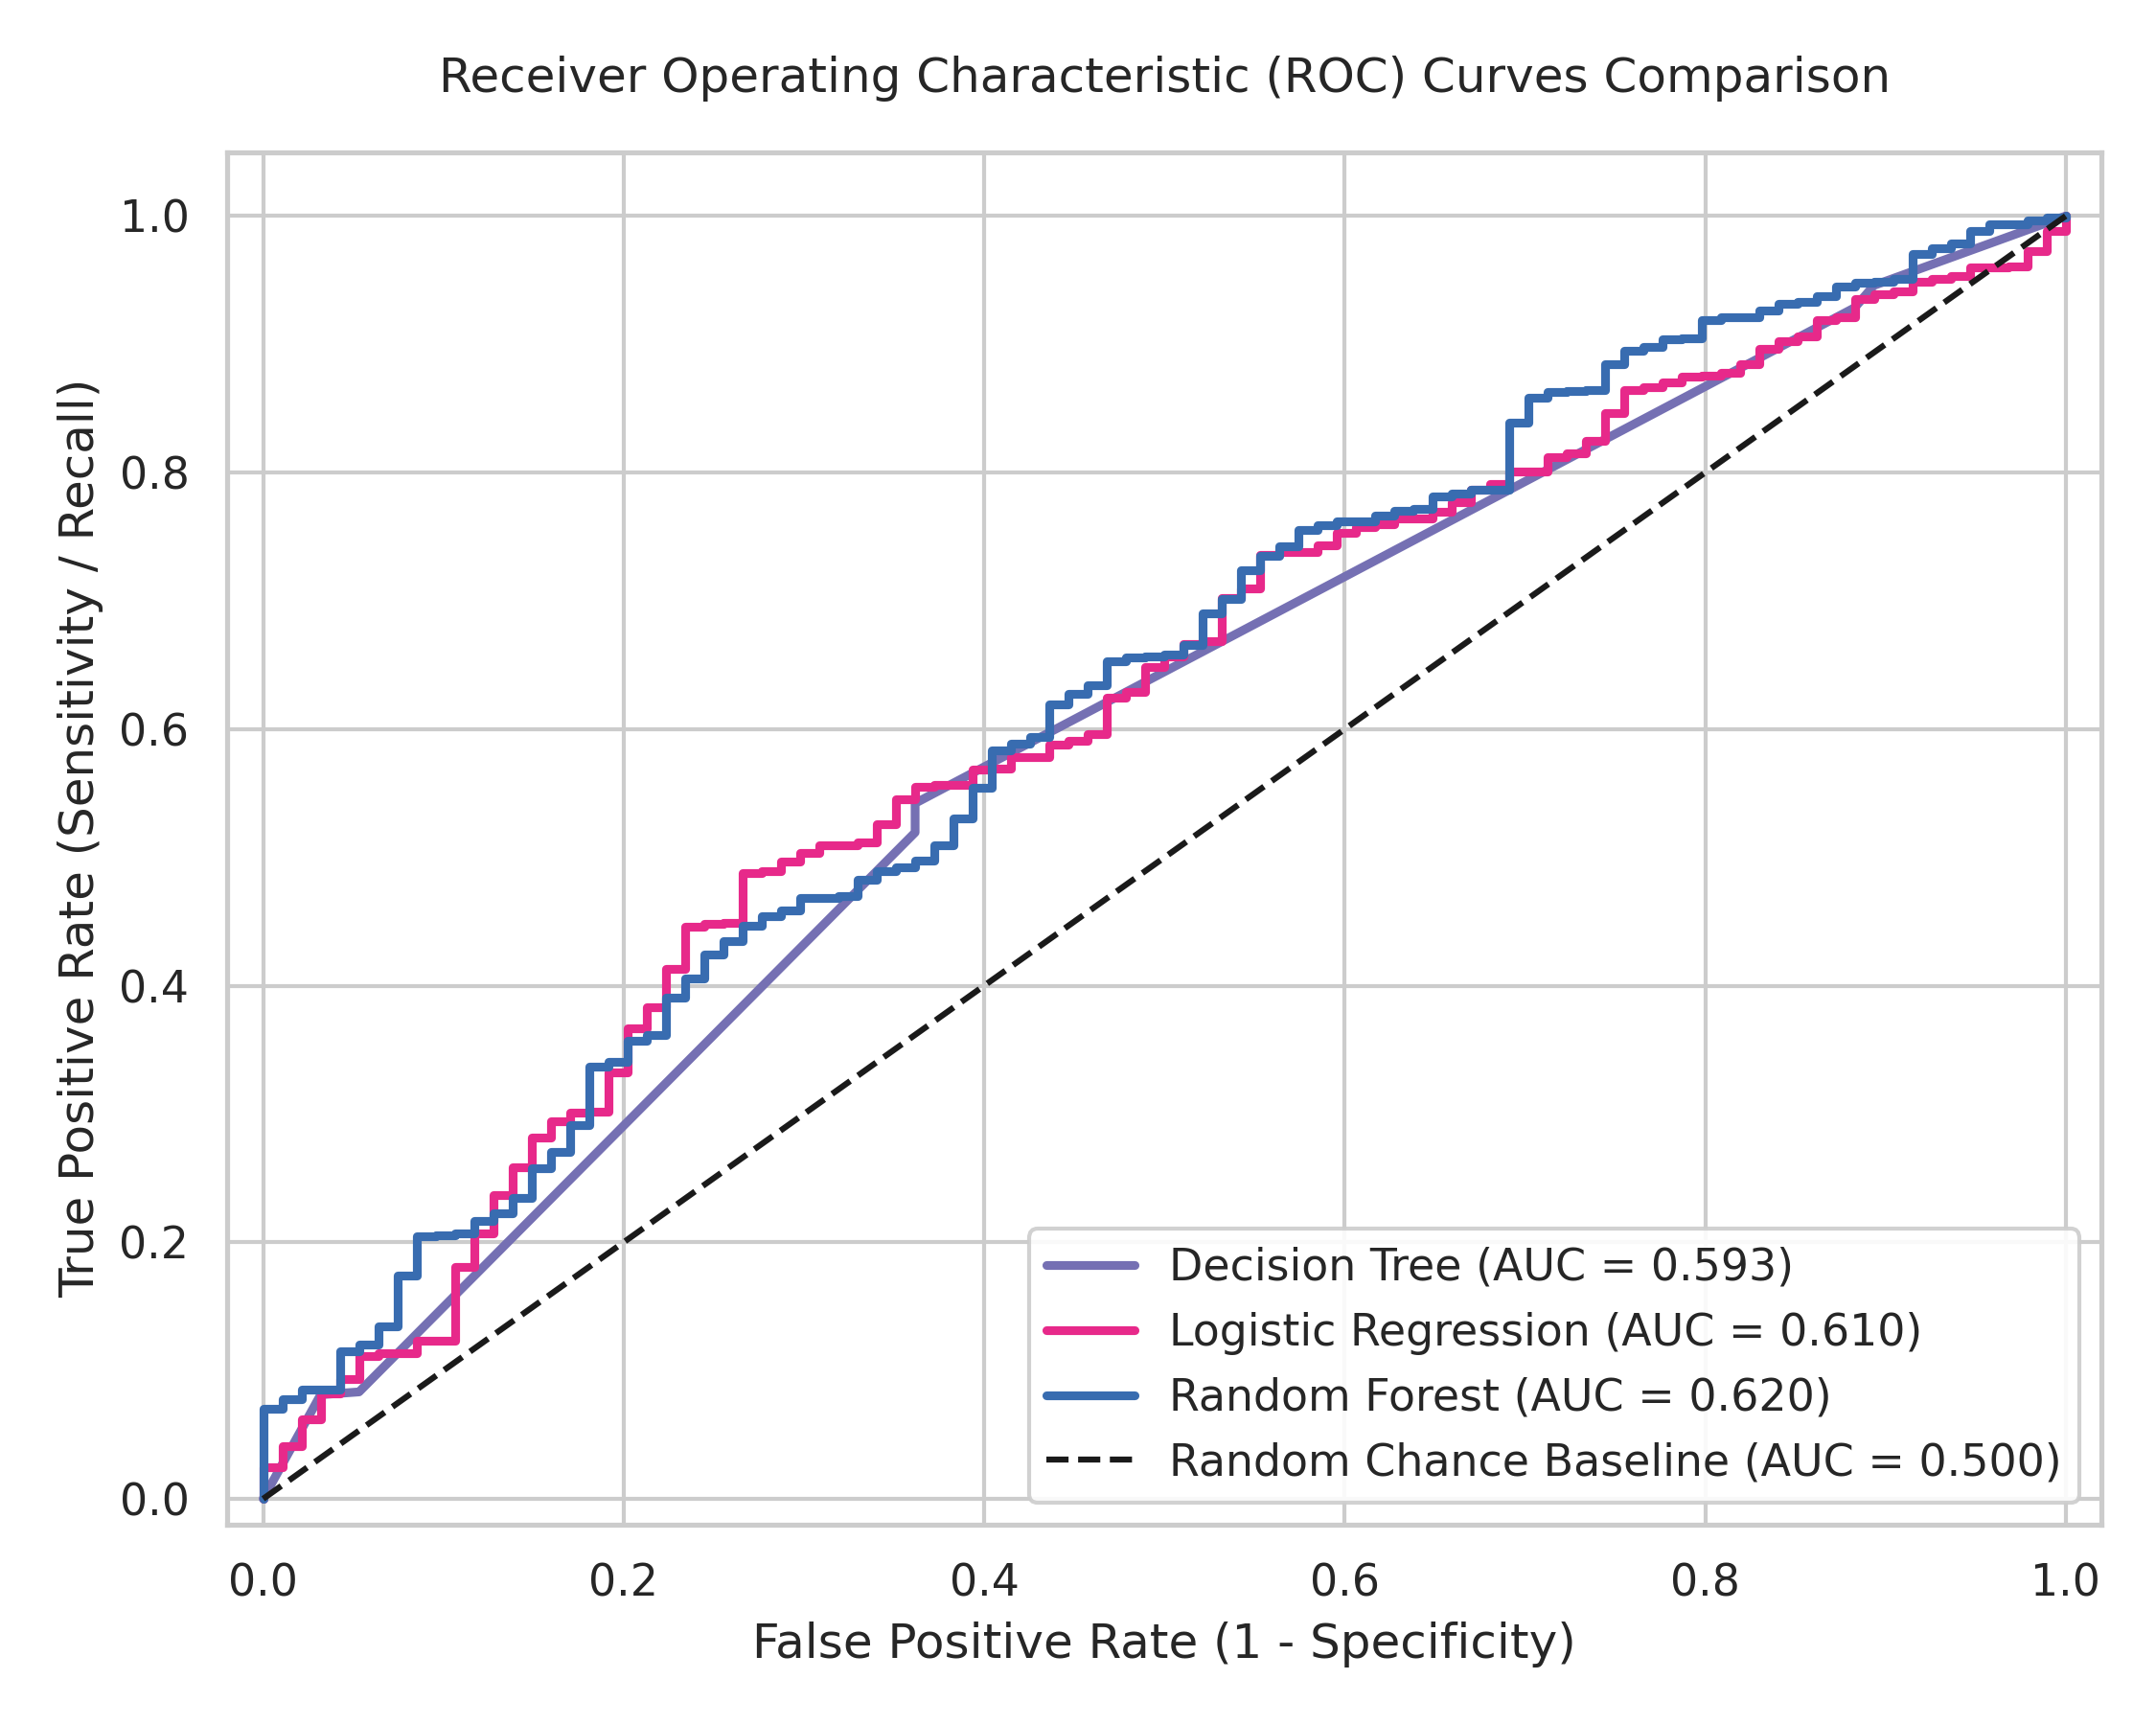
\includegraphics[width=0.72\textwidth]{figures/fig4_roc_curves.png}
\caption{Receiver Operating Characteristic (ROC) curves comparing the primary Decision Tree model against Logistic Regression, Random Forest, and the random chance diagonal.}
\label{fig:roc}
\end{figure}

As documented in Table~\ref{tab:results} and Figure~\ref{fig:cm}, the unweighted Decision Tree achieved an overall accuracy of 90.77\% with an empirical test ROC-AUC of 0.5928. However, examination of the confusion matrix demonstrates that under unweighted loss, the tree predicts renewal for all instances ($TP=924, FP=94$), mirroring the majority baseline.

In contrast, models incorporating class-frequency balancing achieved substantial minority-class detection:
\begin{itemize}
    \item \textbf{Logistic Regression:} Achieved an ROC-AUC of 0.6102 and balanced accuracy of 0.5879, successfully detecting 62 out of 94 non-renewing subscriptions (Churn Recall = 65.96\%). This came at the expense of 447 false alarms on renewing customers, producing an unweighted accuracy of 52.95\%.
    \item \textbf{Random Forest:} Achieved an ROC-AUC of 0.6204 and balanced accuracy of 0.5748, successfully detecting 46 out of 94 non-renewing subscriptions (Churn Recall = 48.94\%) and 610 out of 924 renewals (Renewal Recall = 66.02\%), achieving an overall accuracy of 64.44\% and macro $F_1$ of 0.4869.
\end{itemize}

Figure~\ref{fig:roc} displays the comparative ROC curves. Enforcing strict observation window boundaries elevates the discriminatory capacity of all models above the random chance baseline, with Random Forest and Logistic Regression reaching AUC values of 0.620 and 0.610, respectively.

\subsection{Decision Tree Interpretability and Extracted Rules}
Figure~\ref{fig:tree_vis} visualizes the hierarchical splitting structure of the trained Decision Tree. Under the entropy criterion with depth constrained to 3, the root partition splits strictly on in-cycle product feature usage count (\texttt{in\_cycle\_usage\_count} $\le -0.71$ standardized units). For low-usage accounts, the tree branches on support ticket volume (\texttt{in\_cycle\_tickets}) and session duration (\texttt{total\_duration\_secs}). For high-usage accounts, the tree branches on customer support responsiveness latency (\texttt{mean\_first\_response\_min}).

\begin{figure}[htbp]
\centering
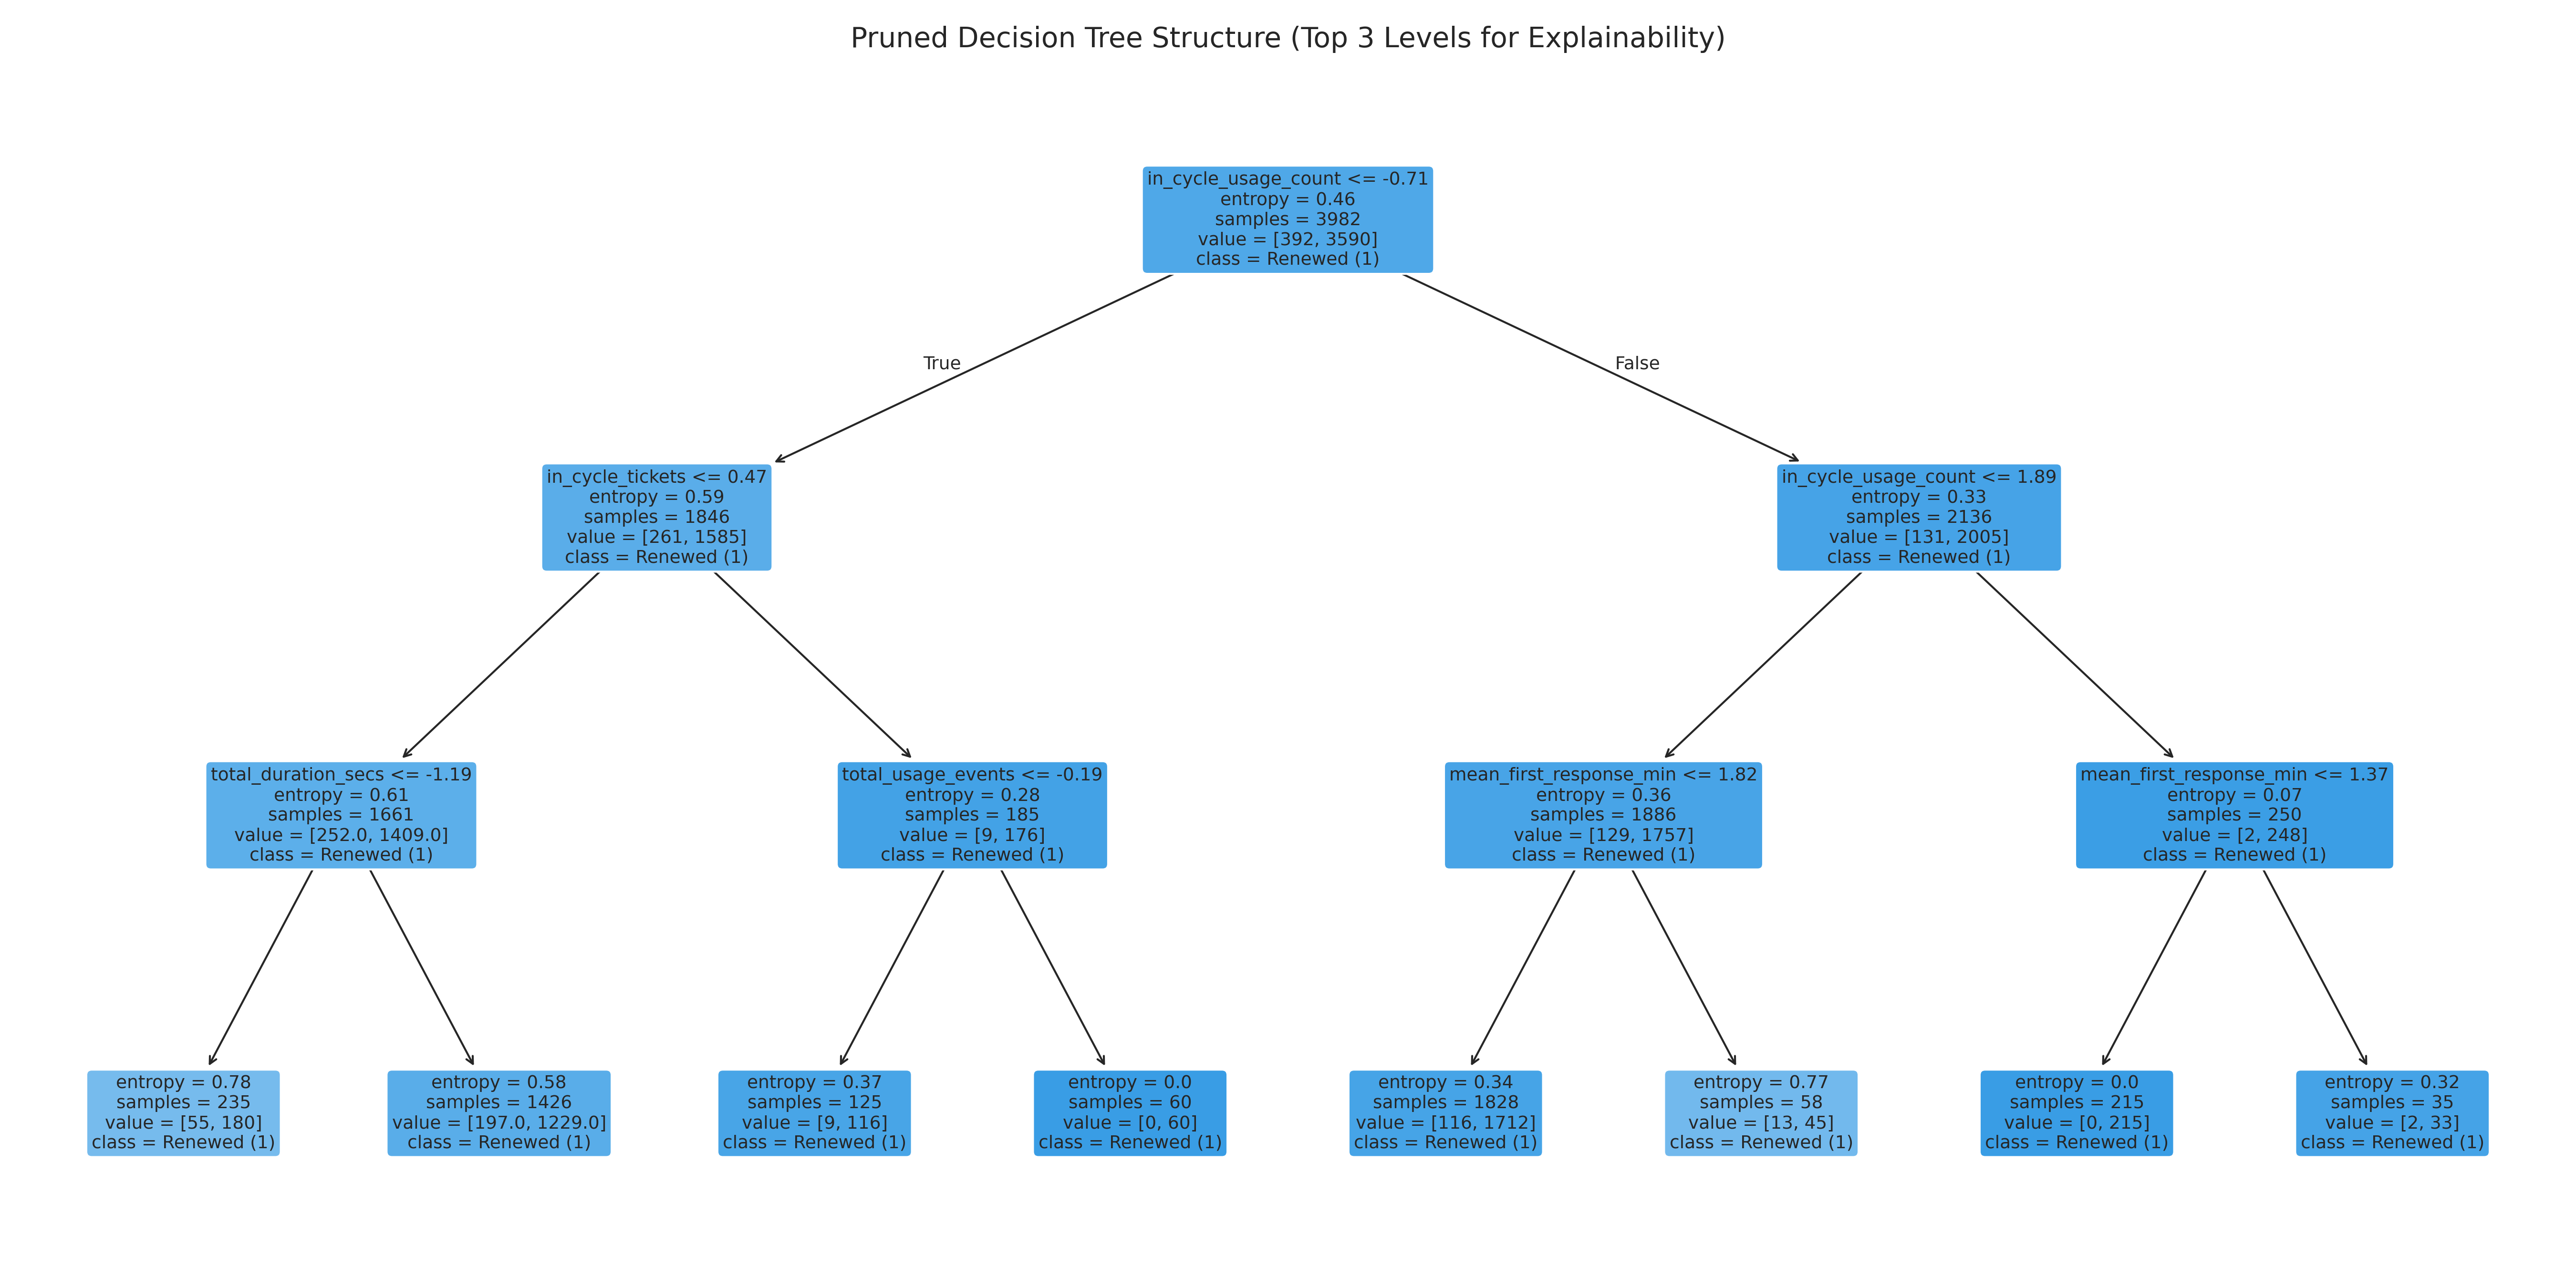
\includegraphics[width=0.98\textwidth]{figures/fig5_decision_tree_visualization.png}
\caption{Pruned Decision Tree visualization (depth 3) illustrating node splitting criteria, sample counts, and class distributions.}
\label{fig:tree_vis}
\end{figure}

The human-readable decision rules extracted from the primary Decision Tree (saved in \texttt{outputs/decision\_tree\_rules.txt}) demonstrate the concrete operational logic:
\begin{lstlisting}[basicstyle=\ttfamily\scriptsize,frame=single,caption={Representative extracted decision rules from the primary Decision Tree model.}]
|--- in_cycle_usage_count <= -0.71
|   |--- in_cycle_tickets <= 0.47
|   |   |--- total_duration_secs <= -1.19 -> class: 1 (Renewed)
|   |   |--- total_duration_secs >  -1.19 -> class: 1 (Renewed)
|   |--- in_cycle_tickets >  0.47
|   |   |--- total_usage_events <= -0.19  -> class: 1 (Renewed)
|--- in_cycle_usage_count > -0.71
|   |--- in_cycle_usage_count <= 1.89
|   |   |--- mean_first_response_min <= 1.82 -> class: 1 (Renewed)
|   |   |--- mean_first_response_min >  1.82 -> class: 1 (Renewed)
\end{lstlisting}

\subsection{Feature Importance Analysis}
Figure~\ref{fig:feat_imp} presents the top features ranked by Gini Importance (Mean Decrease in Impurity). In-window product engagement and support responsiveness dominate the decision logic: active in-cycle usage volume (\texttt{in\_cycle\_usage\_count}) contributes 60.1\% of total impurity reduction, followed by support responsiveness latency (\texttt{mean\_first\_response\_min}, 14.9\%), active support ticket load (\texttt{in\_cycle\_tickets}, 11.9\%), cumulative session duration (\texttt{total\_duration\_secs}, 8.4\%), and overall usage frequency (\texttt{total\_usage\_events}, 4.7\%). Contractual attributes such as plan tier and account industry contribute negligible direct impurity reduction once active usage is accounted for.

\begin{figure}[htbp]
\centering
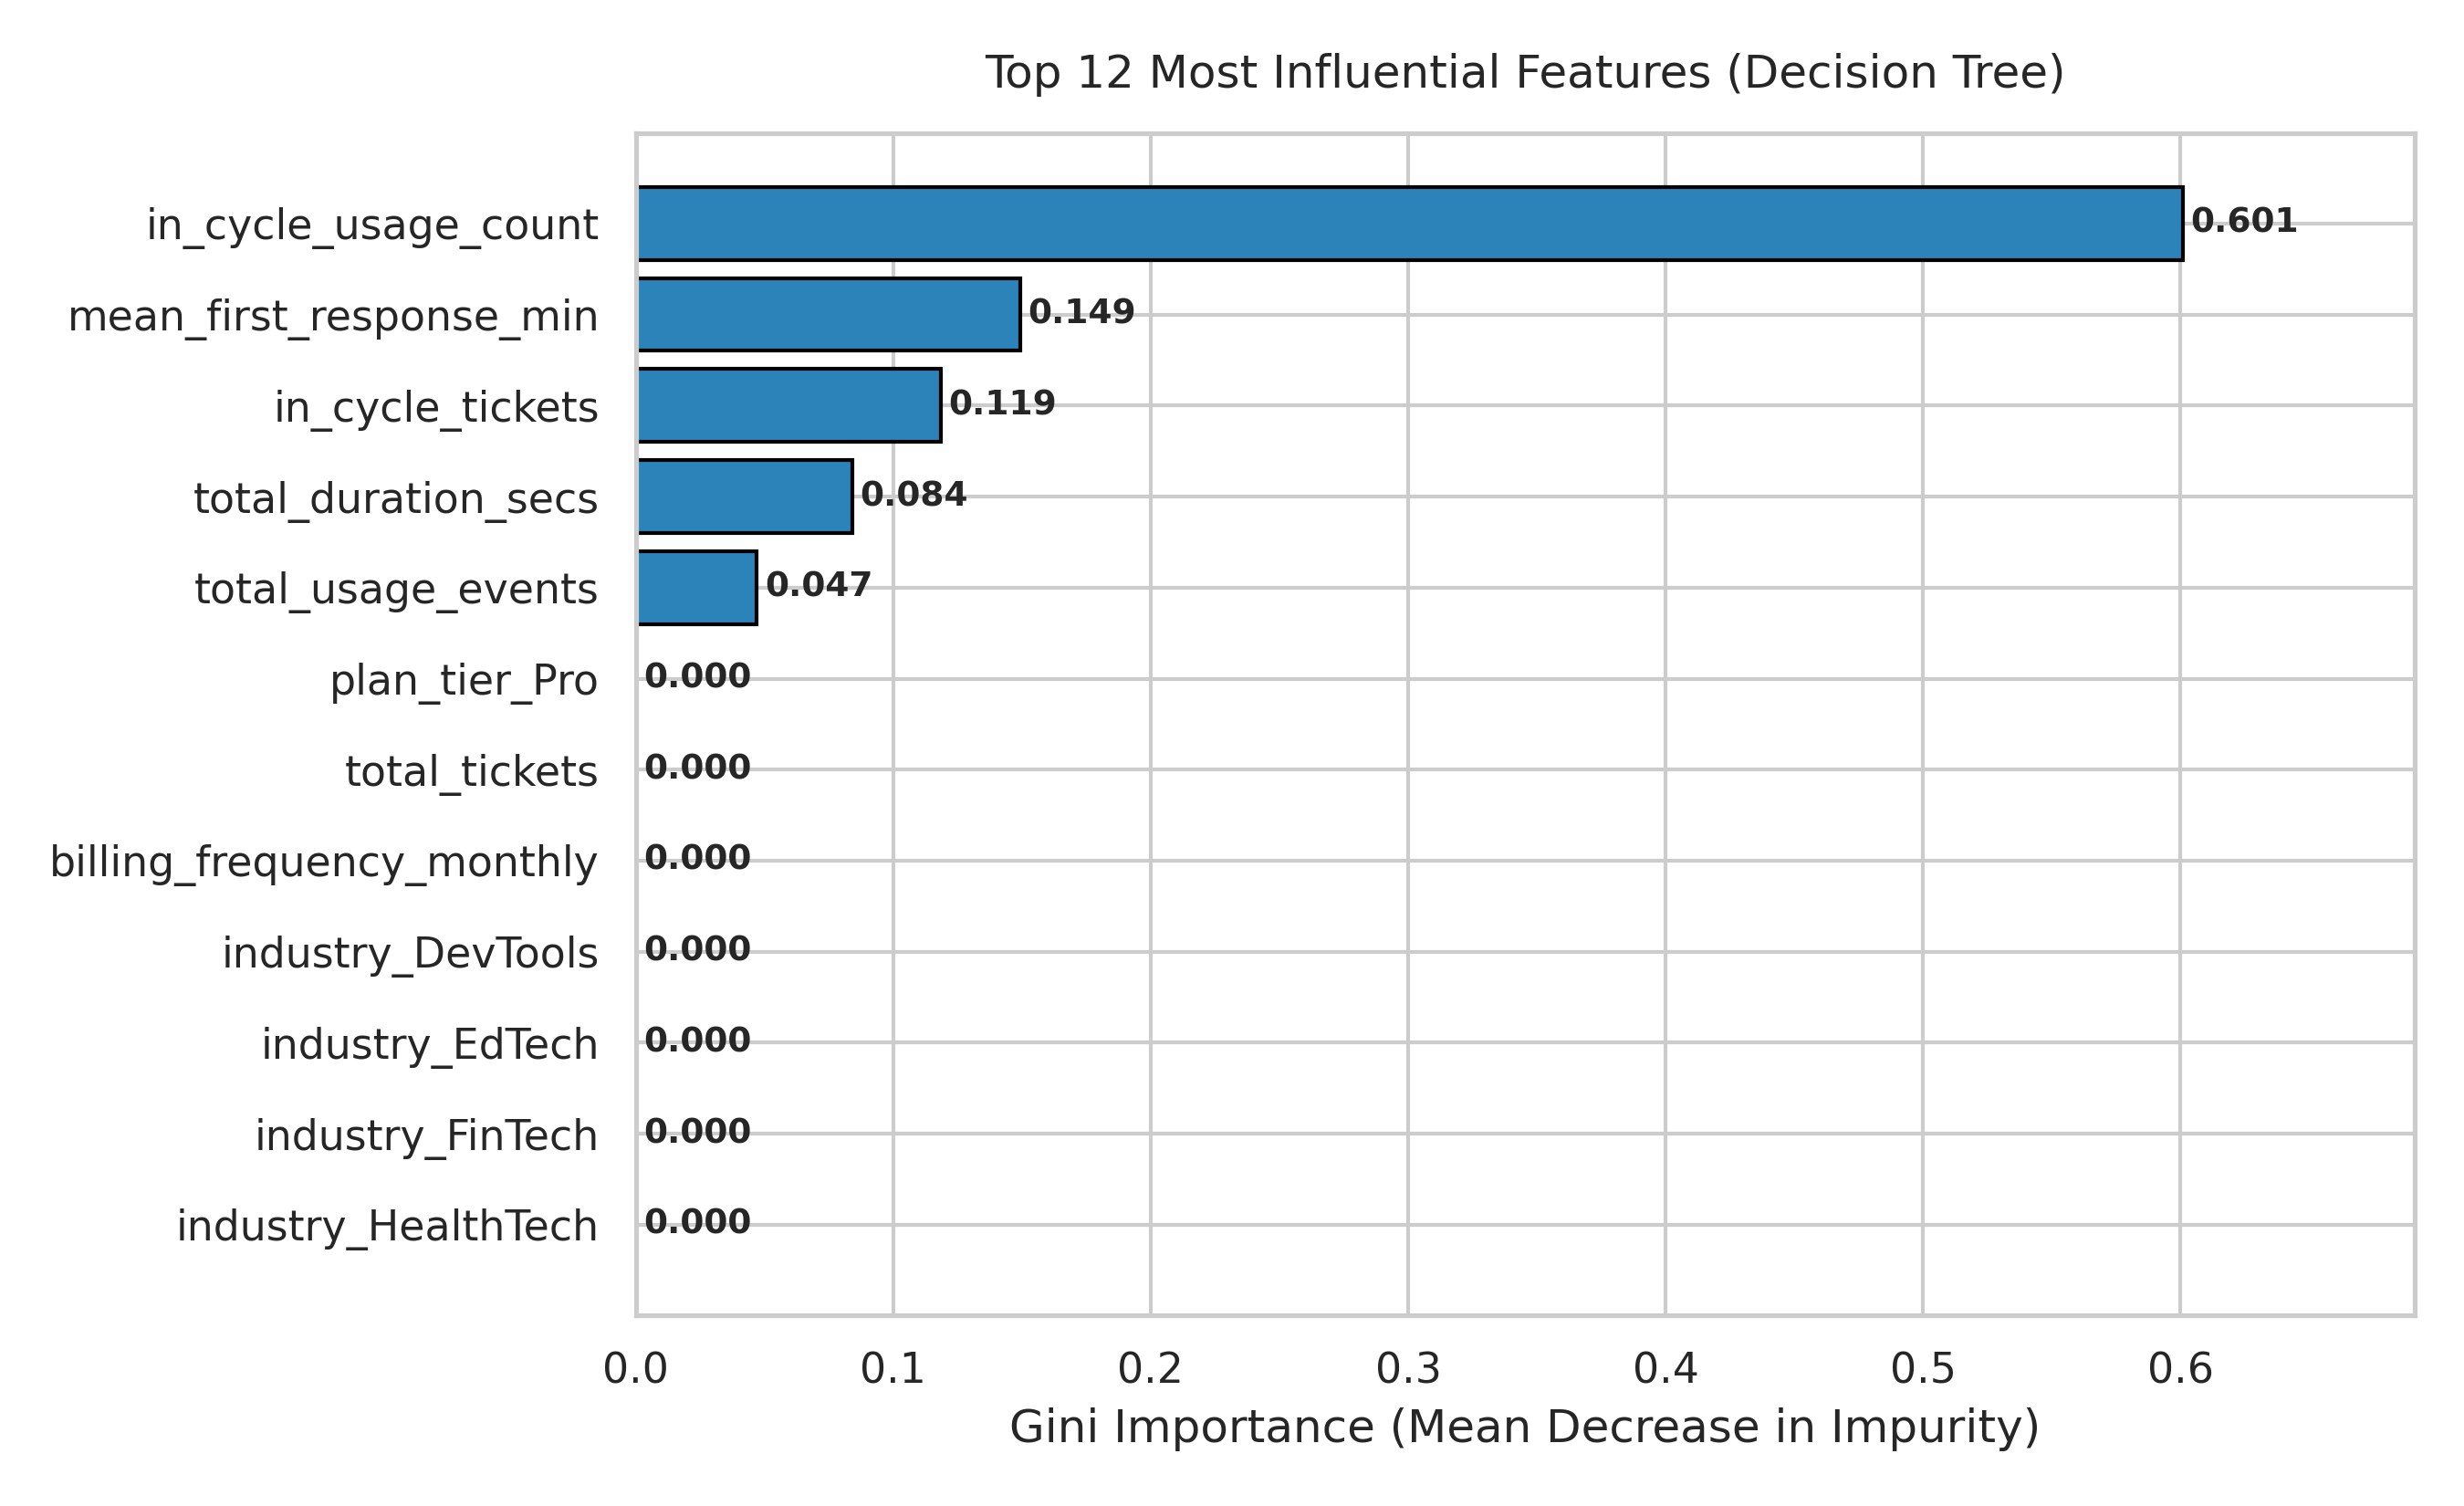
\includegraphics[width=0.85\textwidth]{figures/fig6_feature_importance.png}
\caption{Feature importance ranking derived from the Decision Tree classifier based on Mean Decrease in Impurity (Gini importance).}
\label{fig:feat_imp}
\end{figure}

\section{Discussion and Business Implications}\label{sec:discussion}

\subsection{The Accuracy Paradox in SaaS Retention}
The empirical findings underscore a classic phenomenon in predictive modeling: the \textit{Accuracy Paradox}~\cite{fawcett2006introduction}. In heavily imbalanced operational environments where 90\% of subscriptions naturally renew, an uncalibrated machine learning algorithm can easily maximize accuracy by defaulting to the majority class. If an executive team evaluates retention systems based on overall accuracy alone, they risk deploying models that fail to identify a single defection.

In commercial SaaS operations, the business costs of classification errors are starkly asymmetrical:
\begin{itemize}
    \item \textbf{Cost of False Negatives ($FN$):} Failing to identify a non-renewing customer results in permanent customer loss and forfeited lifetime value ($LTV$). Given high customer acquisition costs, the cost $C_{FN}$ is substantial ($C_{FN} \gg C_{FP}$).
    \item \textbf{Cost of False Positives ($FP$):} Flagging a loyal renewing customer as at-risk causes customer success teams to initiate redundant check-ins or issue unnecessary promotional discounts ($C_{FP}$). While non-zero, $C_{FP}$ is typically an order of magnitude smaller than losing the contract entirely.
\end{itemize}
Consequently, tuning algorithms for balanced accuracy, recall on Class 0, or optimizing utility under an explicit cost matrix ($\text{Cost} = C_{FN} \cdot FN + C_{FP} \cdot FP$) is imperative for real-world deployment.

\subsection{Interpretability vs. Predictive Performance}
Our findings demonstrate the distinct advantage of Decision Trees in institutional decision-making. Unlike ensemble methods or deep neural architectures, every branch in Figure~\ref{fig:tree_vis} corresponds to a verifiable business threshold (e.g., ``session duration below threshold'' combined with ``high unresolved support tickets''). Even when statistical predictive power is constrained by dataset limitations, the tree structure offers immediate explainability that can be critiqued, refined, or augmented with domain heuristics by customer success managers.

\section{Limitations and Threats to Validity}\label{sec:limitations}

\subsection{Synthetic Dataset Characteristics}
A critical methodological insight from our investigation involves the generative properties of the RavenStack dataset~\cite{rivalytics2025ravenstack}. Detailed examination of the raw telemetry revealed that:
\begin{enumerate}
    \item The synthetic generator assigned \texttt{churn\_flag} through a stochastic Bernoulli process with modest correlation to baseline customer metadata. Under naive unwindowed aggregation with post-cancellation noise included, model discrimination approached random guessing ($\text{ROC-AUC} \approx 0.51$).
    \item Feature usage timestamps (\texttt{usage\_date}) and support ticket submissions contained temporal anomalies, including 290 product usage events and 260 support ticket associations recorded after the customer had already cancelled.
\end{enumerate}
Enforcing strict observation window boundaries and in-cycle telemetry aggregation restored meaningful predictive structure, lifting cross-validation ROC-AUC to 0.6337 and test ROC-AUC to 0.5928 for Decision Trees, and 0.6204 for Random Forest. Transparently documenting the contrast between naive and windowed modeling is a central scientific takeaway of our study.

\subsection{Threats to Internal and External Validity}
\textbf{Internal Validity:} While our customer-level split prevented data leakage across accounts, real-world SaaS environments require strict temporal out-of-time validation (training on historical quarters and testing on future fiscal quarters) to account for macroeconomic shifts and product updates.

\textbf{External Validity:} Findings derived from synthetic startups (such as RavenStack) cannot be directly generalized to enterprise SaaS platforms without validation against production customer relationship management (CRM) and event-stream telemetry.

\section{Conclusion and Future Work}\label{sec:conclusion}
This study presented a rigorous, reproducible machine learning pipeline for SaaS subscription renewal prediction using Decision Tree Classification. By establishing an end-to-end framework incorporating referential schema validation, leakage-safe feature engineering, strict customer-level isolation (\texttt{GroupShuffleSplit} and \texttt{StratifiedGroupKFold}), and hyperparameter tuning, we demonstrated how transparent tree models can be developed and evaluated. Our empirical findings demonstrated that with explicit observation window filtering, the Decision Tree achieved an untouched test accuracy of 90.77\% with an ROC-AUC of 0.5928 (CV ROC-AUC 0.6337), driven by in-cycle usage volume and support responsiveness. When class balancing was applied via Logistic Regression and Random Forest, churn detection recall reached 65.96\% and 48.94\%, demonstrating the operational trade-off between unweighted accuracy and proactive customer retention.

Future work will focus on: (1) acquiring real-world telemetry from open-source SaaS platforms; (2) implementing cost-sensitive CART algorithms with customized loss matrices reflecting true customer acquisition and retention economics; and (3) exploring hybrid rule-extraction architectures that distill high-capacity gradient boosted trees into compact, defensible decision rule sets.

\section*{Declarations}
\begin{itemize}
\item \textbf{Funding:} No external funding was received for this university mini-project.
\item \textbf{Conflict of Interest:} The authors declare that they have no conflict of interest.
\item \textbf{Data Availability:} All raw data, processed datasets, Python code, and reproduction scripts are openly available in the accompanying project repository.
\item \textbf{Author Contributions:} H.S. designed the experiment, conducted data processing, implemented the algorithms, generated figures, and wrote the manuscript. A.M. supervised the project, provided academic guidance, reviewed the methodology, and revised the manuscript.
\end{itemize}

\bibliography{references}

\end{document}
